\chapter{Skin recognition}
    Earlier, we described why liveness detection is an important part
    of a face recognition system and why it could greatly improve security.
    In our research, we focused on using light reflectiveness to recognize skin on photos.
    This idea comes from the fact that every material has its own, unique spectrum.
    % [TODO: LINK NEEDED]
    Different types of human skin reflect visible light very differently
    \cite{hsreflectance},
    but those differences become smaller when going further into infrared wavelengths
    \cite{visinfra} \cite{toyotaskin}, which is why we decided to use infrared light
    in our experiments.
    Ideally, we would like to have a spectrometer in a mobile device,
    which has been done before \cite{spectrometerphone}.

    Additionally, with the information of which pixel contains human skin,
    it would be possible to use this to remove the background from face
    photos \cite{colorstudy}.
    As described in a later chapter, this is an important part of face recognition,
    and is currently done using methods based on machine learning, which are usually
    rather slow.
    Using skin detection could significantly improve the performance of background
    removal.

    \section{Technical aspect -- how does a camera work?}
        To think about the security aspect of skin detection,
        it is critical to understand how image sensors works.
        The most common sensors are \textit{CCD} (\textit{charge-coupled device})
        and \textit{CMOS} (\textit{complementary metal-oxide-semiconductor}) \cite{mostcommons}.
        Due to better quality, as well as sensitiveness, for security reasons
        it probably would be better to use CCD.
        However, both matrices have same problem -- limitations on wavelength sensitivity.
        Such sensors are sensitive to wavelengths approximately up to 1050nm
        \cite{imagesensorsmax},
        which may be a serious limitation as human skin has more undifferentiated
        characteristics in greater wavelengths.
        Therefore looking for the the best possible skin detection method,
        it may be convenient to assume that other type of light sensitive matrices
        are in reach of an inventor.
        Nevertheless, we were limited to very common cameras.

        We are describing one possible realization, but keep in mind that
        there are more solutions, which we did not find useful in our problem.

        \subsection*{Monochrome}
            As an image sensor is a matrix built from many small photodiodes,
            it is natural to create a monochromatic image.
            Because photodiodes do not distinguish different
            wavelengths, only light intensity, it is hard
            to measure light reflectiveness.
            The only possible way to do that is to
            take a separate picture for every wavelength.
            It is not easy, as you have to
            provide your own lighting and somehow remove
            light coming from other sources.
            Also, all pictures have to be made in
            a~very short time interval, as the subject
            cannot move between shots.

        \subsection*{Multispectral imaging}
            Multispectral imaging is a way to measure every wavelength intensity
            in one picture, so it is an answer to the problem of the object moving.
            Probably the easiest way to describe it is to look at an RGB camera
            (with a Bayer-like filter \cite{bayerfilter}).
            There, every photodiode is responsible for exactly one color,
            where as color we understand a wavelength interval (it is important
            to understand that we can consider any wavelength interval as one color).
            The result picture is built from small squares (mostly $2 \times 2$)
            of photodiode matrix data.
            In fact, there may be more than just three colors.
            For example, you may find a camera which can see two types of green.
            Usually, in the end everything is converted to the well-known RGB format.

            \begin{figure}[H]
                \caption{RGB image sensor matrix with two types of green -- sensors arrangement.}
                \centering
                \includegraphics{RGB-matrix}
                \label{fig:RGB-matrix}
            \end{figure}

            Each sensor reports what is the light intensity to the camera, which then
            reports that intensity and which color that sensor filters to the software.

            One of the possible realizations of reducing the range
            of light visible through a sensor is to take a standard image sensor, which
            may see the full spectrum of light (CCD -- $350$-$1050$nm
            \cite{imagesensorsmax}), and place filters
            in the way, so that only specific light will reach the chosen photodiode.

            \begin{figure}[H]
                \caption{Visualization of a filtering mechanism.}
                \centering
                \includegraphics[scale=0.40]{RGB-filter}
                \label{fig:RGB-filter}
            \end{figure}

        \subsection*{Hyperspectral imaging}
            Hyperspectral imaging is creating pictures using a camera with the
            capability to distinguish a large amount of colors
            (even hundreds or thousands) instead of just a few.
            It would be very helpful to have one in a skin detection device,
            but it would be impractical to put a hyperspectral camera in a mobile phone.

    \section{Technical aspect -- how can it be created?}
        As we now know how a camera works, we can distinguish two ways of
        building a skin-detecting mobile device.
        \subsection*{Monochrome}
            We can work without filters (or with one for the whole camera),
            but then we have to take a picture for every wave length.
            Also, we need one diode producing the exact wavelength we want.
            It is an easier method to implement in a phone, but taking pictures
            would have to be very fast.

            The biggest advantage of that solution is the possibility of lighting
            with different LEDs in random moments of time, so hackers
            would not be able to play with their own diodes to modify the results.

        \subsection*{Multispectral imaging}
            There is also a possibility to use filters with specific infrared colors.
            But it is important here to avoid standard smoothing algorithms used
            in cameras.
            The real light intensity from every sensor is needed,
            without any postprocessing.

    \section{Our attempts}

        \subsection{Detecting reflectiveness using Kinect}
            Our first idea was to use a Kinect v2 depth and infrared camera to detect
            how well does a surface reflect light.
            Kinect v2 cameras have their own source of infrared light and they make
            a very good job at filtering other sources of light.
            So, for each pixel on the infrared image, we know how much light coming
            from the Kinect's light emitter was reflected in that particular place.
            Also, Kinects are depth cameras, which additionally gives us the information
            on how far away from the camera is the object visible on that pixel.

            Since the source of light is in the same device as the camera, the distance
            seen on the depth image is also the distance from the light emitter.
            This is an important observation, because we know how distance affects how
            much light arrives at a particular place. % might need a better wording
            If we have a source of light that, at a given distance, lights up a
            1cm $\times$ 1cm square of a flat surface with a particular amount
            of light, then at double that distance it will light up a 2cm $\times$ 2cm
            square with the same amount of light, which means that the same amount
            of light is distributed over a 4 times larger surface, so the
            intensity of light has to be 4 times lower than before.

            With those observations, we took pairs of IR and depth images, and for each
            pixel calculated a new value of $ir\_intensity \cdot depth \cdot depth$,
            which should estimate how well light was reflected at that point,
            regardless of distance from the camera.

            \begin{figure}[H]
                \caption{An unprocessed IR photo, and an image calculated using
                the method described above.}
                \centering
                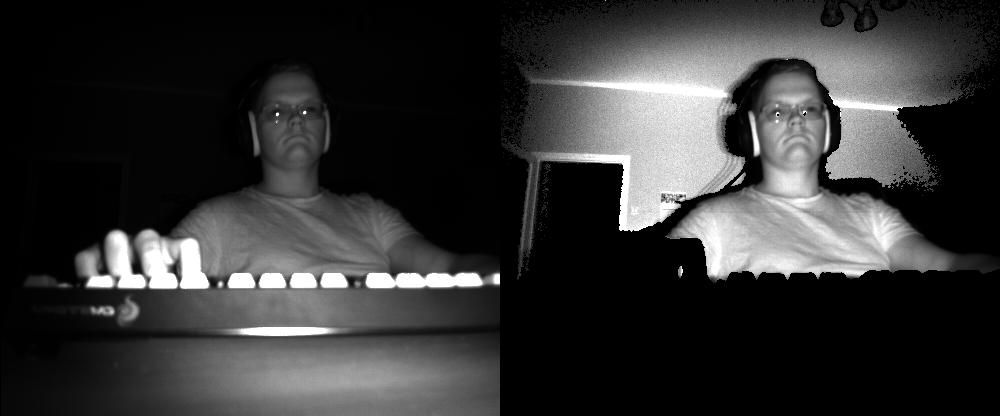
\includegraphics[width=0.7\textwidth]{skin_kinect_1}
                \label{fig:skin_kinect_1}
            \end{figure}

            As seen on figure \ref{fig:skin_kinect_1}, we have accidentally created
            a night vision camera (please note that some of the black areas are there
            because Kinect cameras do not give depth data for objects closer than 50cm)
            -- but this means that our idea is to some extent working, because the point
            of it was to make objects in the distance indistinguishable from those close
            to the camera.

            However, one thing that is not considered in that method is that objects
            can also be at different angles to the camera.
            A sheet of paper perpendicular to the source of light will reflect more
            light to the Kinect than it would reflect if it was at a 45 degrees angle.

            \begin{figure}[H]
                \caption{Three IR images processed with the described method, with a
                manually determined interval of values marked red.}
                \centering
                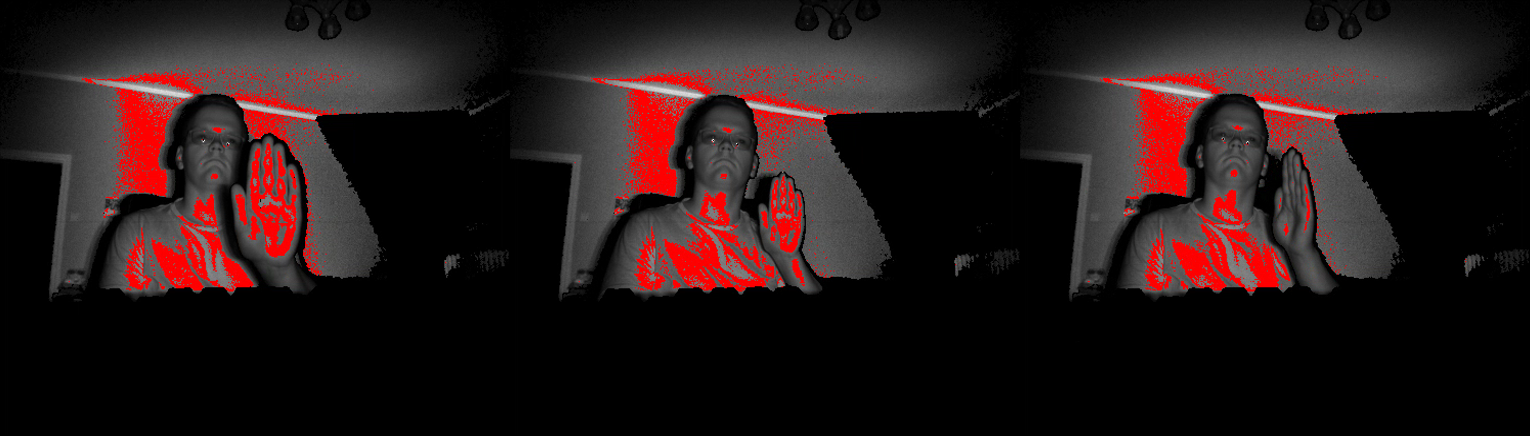
\includegraphics[width=\textwidth]{skin_kinect_2}
                \label{fig:skin_kinect_2}
            \end{figure}

            We have manually selected an interval of values and marked them red, which
            can be seen on figure \ref{fig:skin_kinect_2}.
            On the first two pictures there, the hand is at the same angle, but at a
            different distance to the camera.
            It is visible that the calculated values remained very close regardless
            of the distance, which was a success.
            However, on the third picture, the hand is at a different angle and
            that changes how it reflects light towards the camera, which makes the values
            different.

            Knowing the depth value and certain properties of the camera, it is possible
            to calculate the 3D coordinates of each pixel.
            We calculated cosine between vectors using the formula
            $\cos(v_1, v_2) = \frac{v_1 \cdot v_2}{||v_1||~||v_2||}$.
            We tried to calculate reflectiveness using two data points:
            how flat is the surface (using neighboring pixels and calculating angles between them),
            and what is its angle towards the camera (using a basis vector).

            With that information, it is possible to calculate the angle towards the
            camera between each two pixels and the camera,
            and then use that value in the method above
            to make it independent of angles.
            However, our attempts to do this were unsuccessful, possibly because the
            depth camera is not precise enough.

        \subsection{Using three infrared wavelengths}
            \subsubsection*{Prototype}
            With the previous method using only one light wavelength (the one emitted by
            Kinect), we decided to take photos using three different wavelengths.
            This gives the opportunity to analyze how does the way the object reflects
            light changes with regard to light wavelength, instead of directly looking
            at how bright a point is.

            To make any research, we had to take three photos of the same object
            reflecting three different wavelengths of infrared light.
            The camera, the infrared light sources, and the photographed object
            had to be in the same position for all of the photos.
            An ideal way to do this would be to use a multispectral camera, but they are
            very expensive and we were not able to use one.

            One possible way to take a photo of how a certain wavelength is reflected
            would be to use a filter that only lets that wavelength to pass through it.
            However, changing filters on the camera between taking photos would take
            a lot of time, which would create a risk of changing the relative position
            of the object and the camera, which is unacceptable.

            We borrowed a mobile phone which had a filter mounted on its front camera
            that allowed various wavelengths of infrared light, but not visible light.
            This opened up the opportunity to take a different approach -- instead
            of filtering the selected wavelength, we want to illuminate the object
            using only that wavelength.

            We purchased diodes emitting light in the following wavelengths:
            850nm, 890nm, 940nm. Those diodes were connected to an Arduino board.
            We used two diodes of each wavelength, and mixed their positions to
            make sure that the centers of sources of light at each wavelength
            are as close as possible.

            \begin{figure}[H]
                \caption{Arduino board with six IR diodes.}
                \centering
                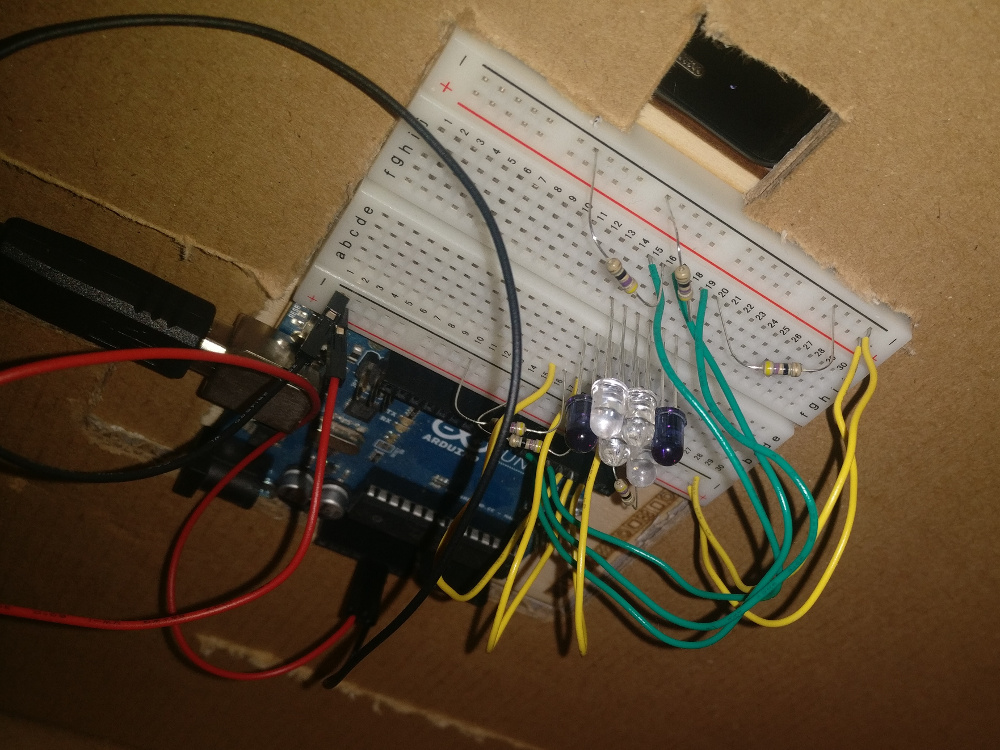
\includegraphics[height=7cm]{arduino_1}
                \label{fig:arduino_1}
            \end{figure}

            Since taking all three photos at the same time would be impossible,
            we stabilized the camera and the diodes by putting them in holes
            in a cardboard box.

            \begin{figure}[H]
                \caption{Outside view of the Arduino board and the camera.}
                \centering
                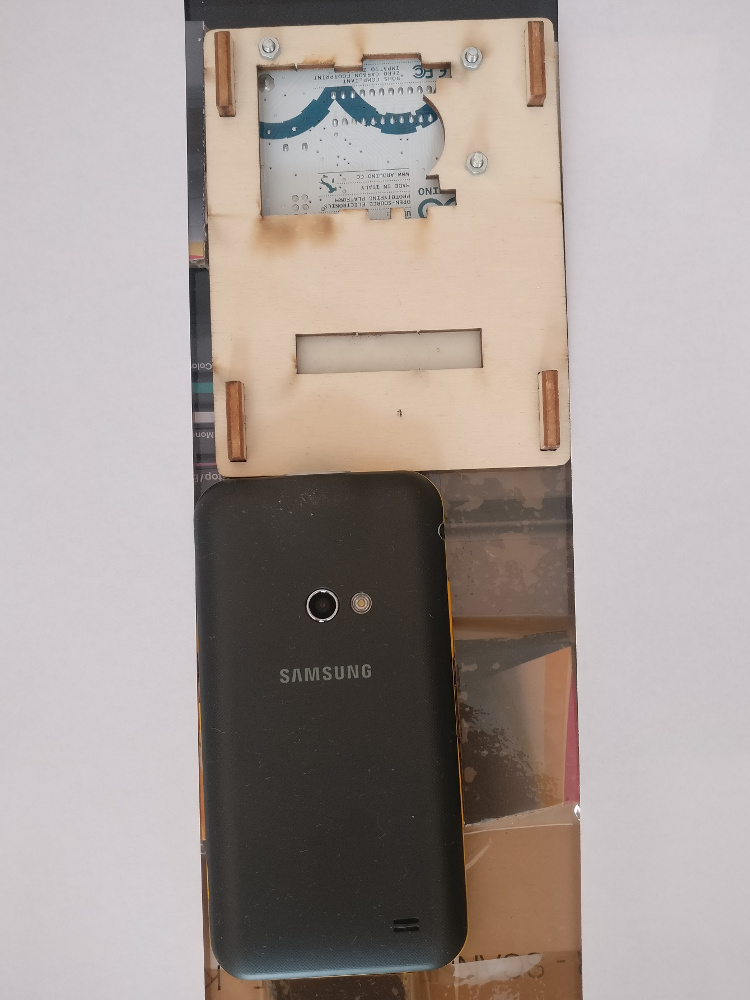
\includegraphics[height=7cm]{arduino_2}
                \label{fig:arduino_2}
            \end{figure}

            With this setup, all that remained to do was to take photos.
            The camera and the phone were stable, but when photographing for example
            a human hand, it might move.
            The photos have to be taken in the smallest possible intervals
            and human interaction can not be required while taking them,
            because that could result in moving the camera or the diodes.

            Turning specific diodes on and off was a rather easy task.
            Arduino is by definition programmable, so we just wrote a program that
            listened to data sent on a USB cable and turned on the requested diode.

            We found an Android app \cite{opencameraremote} designed to take photos
            remotely when commanded so from another phone with a special pilot app.
            It is open source, so we read its source and found out that it just sends
            simple LAN broadcast messages.

            With this information, we were able to write a Python script that did the
            following:

            \begin{itemize}
                \item connect to Arduino through USB, turn on 850nm diodes
                \item wait 0.75 seconds
                \item send a broadcast message to take a photo
                \item wait 0.75 seconds
                \item turn on 890nm diodes
                \item wait 0.75 seconds
                \item take a photo
                \item ... -- analogical procedure to take a photo with 940nm light
            \end{itemize}

            Since we were using only the front camera from a relatively old phone,
            we had to take a 1.5 seconds break between each photo -- otherwise
            there was a significant chance of the camera app not catching one of the
            broadcasted commands and taking only two photos.
            The time between the first and last of three photos was 3 seconds,
            and that was an acceptable delay to make sure that the photographed
            object was in a stable position.

            \begin{figure}[H]
                \caption{Photos taken with 850nm, 890nm, and 940nm light respectively.}
                \centering
                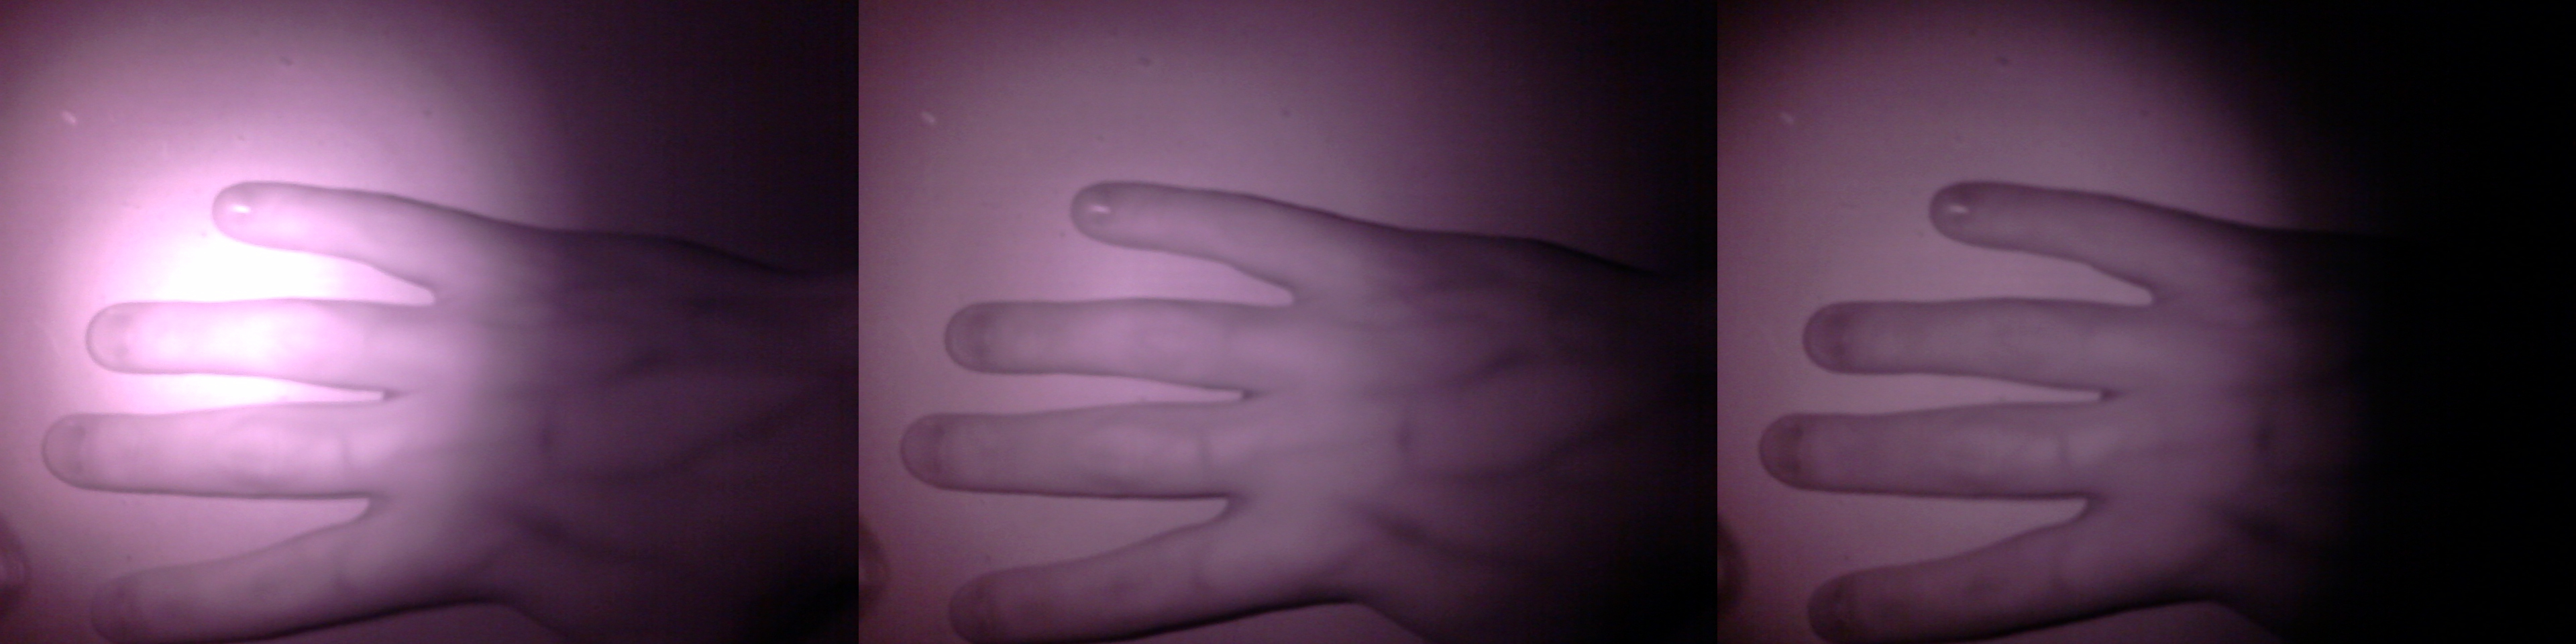
\includegraphics[width=\textwidth]{ir_photos}
                \label{fig:ir_photos}
            \end{figure}

            \subsubsection*{Detecting skin -- preprocessing}
                As we only had a phone camera (with a not-fully-known filter),
                our input was a picture-matrix
                in which every pixel was a nine elements tuple.
                In fact, values there were not independent, because
                for almost every pixel in all JPEGs,
                $R \approx B \approx 2 \cdot G$ occured.
                Therefore, using all that data would only cause overfitting,
                instead of actually improving the model.

                We had many preprocessing ideas, all of which were focused
                on using every pixel independently.
                The one with the best results was taking a few values from each of three pictures
                and calculating differences concatenated with the basic vector (best results for
                random forest, SVM worked best with vectors normalized to unary vectors).
                There is a chance to improve the preprocessing by using more than one pixel,
                but we were focused on getting more reliable results
                (taking an average of adjacent pixels would make it easier
                by reducing the amount of anomalies).

            \subsubsection*{Detecting skin -- models}
                Unfortunately, handmade algorithms to detect skin failed,
                so we decided to use machine learning.
                We prepared an image mask for a picture of a hand,
                which provided information to the algorithm
                about which pixels are skin and which are not.

                \begin{figure}[H]
                    \caption{Example of a manually made skin mask.}
                    \centering
                    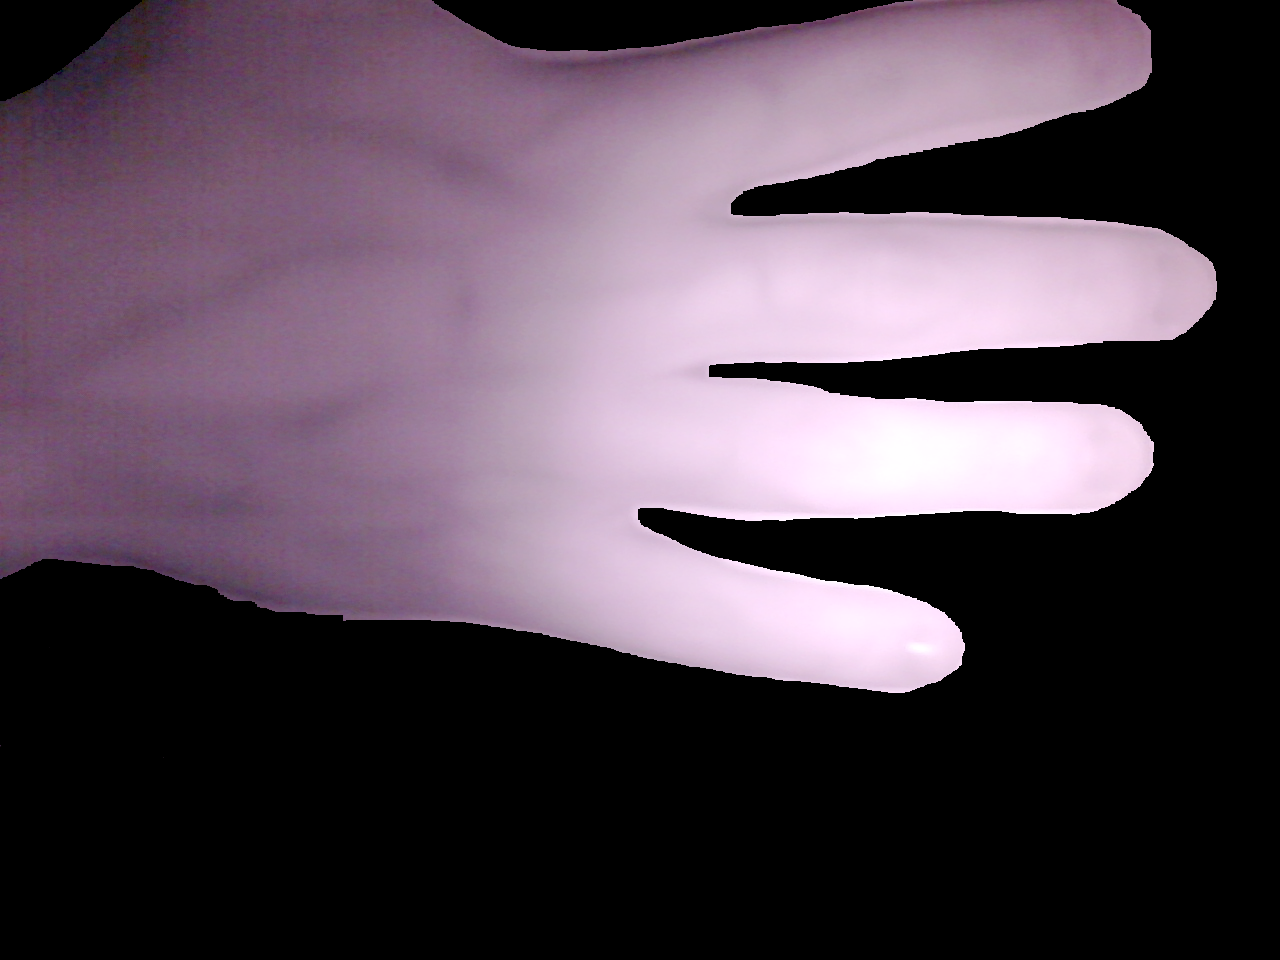
\includegraphics[width=7cm]{A_mask}
                    \label{fig:A_mask}
                \end{figure}

                We used \texttt{scikit-learn} to test different models.
                We hoped that SVM would work well, and with a
                linear kernel it did show some promise.

                 \begin{figure}[H]
                    \caption{SVM without keeping only the well-lit area of the picture.}
                    \centering
                    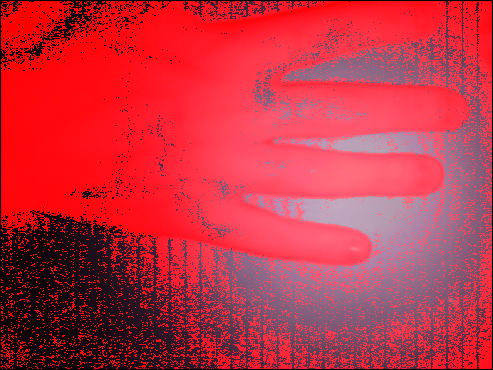
\includegraphics[width=7cm]{svm_no_cut}
                    \label{fig:svm_no_cut}
                \end{figure}

                However, Random Forest achieved better results, as seen on the
                images below.

                  \begin{figure}[H]
                    \caption{Skin detection with SVM using preprocessed data.
                    The first two pictures come from the learning set, others
                    are from the test set.}
                    \centering
                    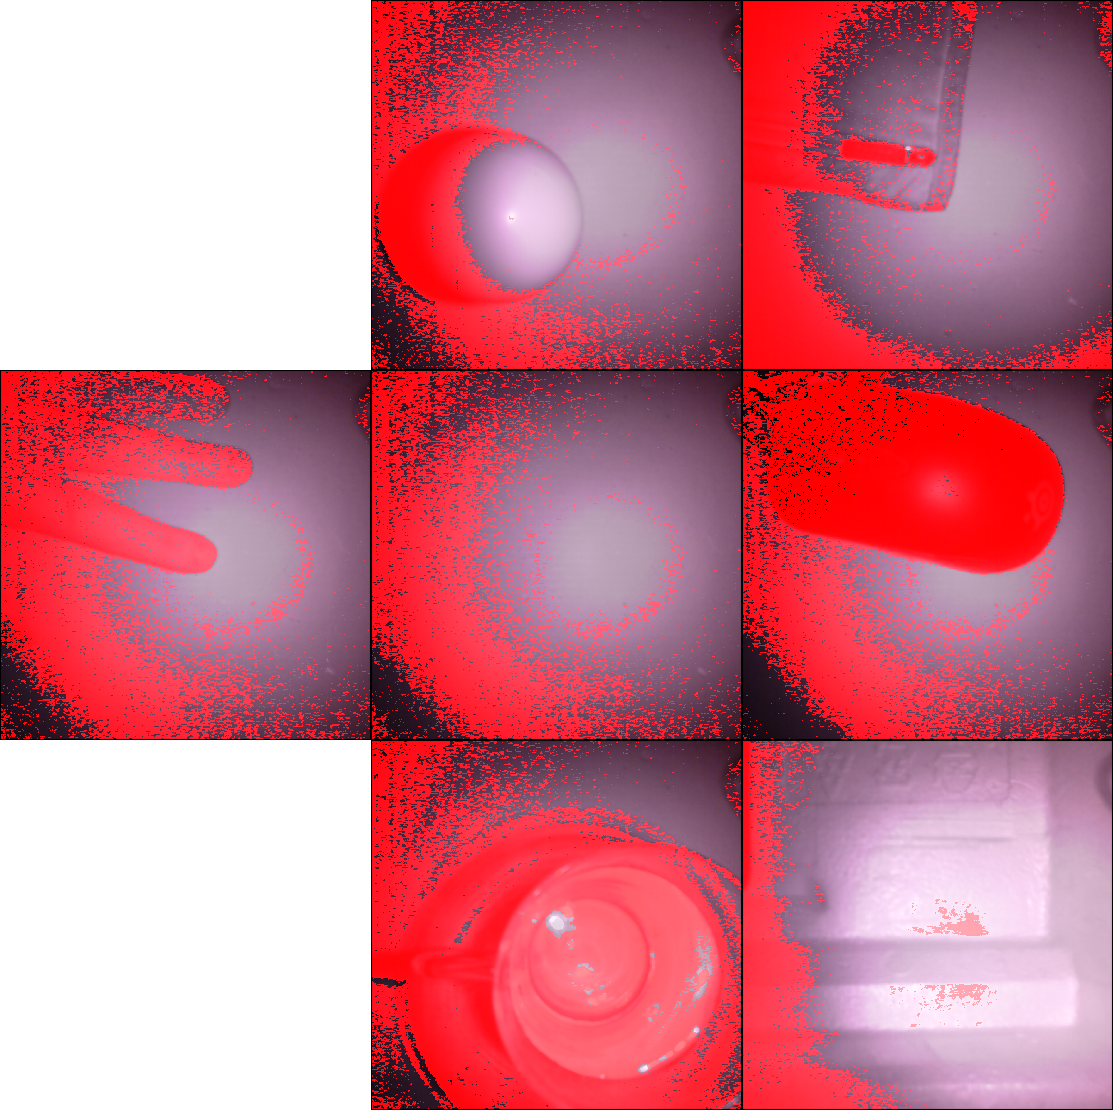
\includegraphics[width=11cm]{svm_skin}
                    \label{fig:svm_good}
                \end{figure}


                \begin{figure}[H]
                    \caption{Skin detection with random forest using preprocessed data.
                    The first two pictures come from the learning set, others
                    are from the test set.}
                    \centering
                    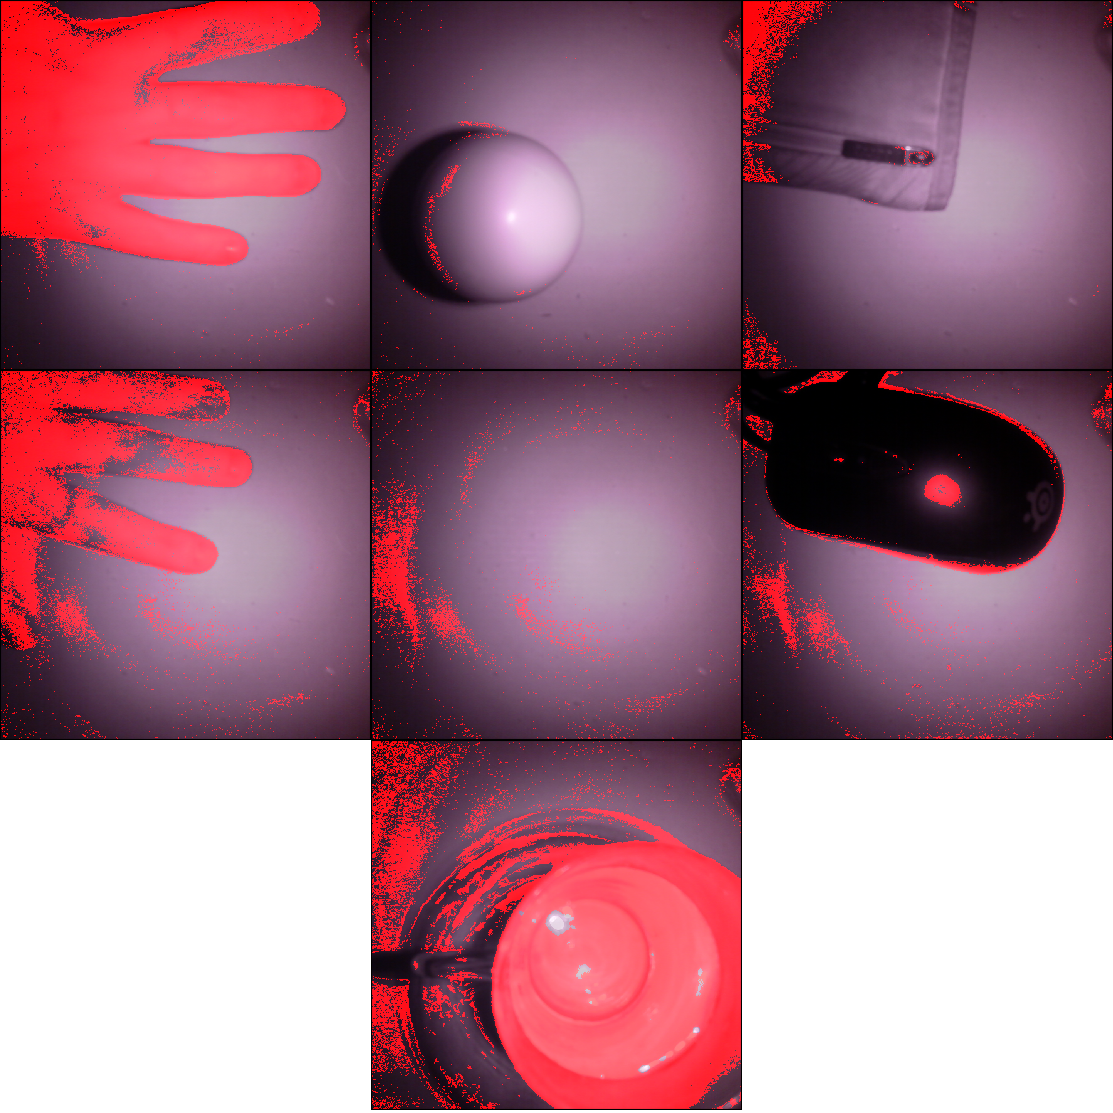
\includegraphics[width=11cm]{rf_good}
                    \label{fig:rf_good}
                \end{figure}

                It is important to notice that a lot of information was lost in the
                picture that we had, as we were not able to take RAW photos or at least
                avoid JPEG compression.
                The consequences of that were visible very well when we tried to
                intentionally overfit out model on some images, and we failed
                because there was not enough information even to overfit.
                Therefore we consider our results better than expected.

                 \begin{figure}[H]
                    \caption{Overfitting random forest on one picture. Wihout and with preprocessing.}
                    \centering
                    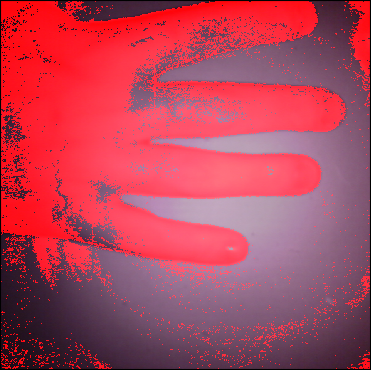
\includegraphics[width=9cm]{rf_overfitting_op}
                    \label{fig:rf_overfitting_op}
                \end{figure}

    \pagebreak

    \section{Results}
        The results achieved by our skin detection were far from perfect,
        however we still think that using infrared photos to analyze surface
        reflectiveness and using that to detect skin is a promising method.
        We were very limited by the low quality and JPEG compressed photos,
        overall lack of high quality hardware, and our lack of knowledge in electronics,
        but were still able to achieve results that visually make sense.
        With more resources, we believe this could increase security of
        face authentication solutions.

        The next big step associated with development of that skin detection
        technology may be using a hyperspectral camera to find a few (for example three
        or four) colors giving greater security, as well as measuring
        quality of that solution with a fixed number of colors.
        Unfortunately, we were not able to use a high quality hyperspectral camera
        to measure possible effectiveness and security of such solution.

    \section{RGB skin detection simulation}
        Because we wanted to have the ability to check how skin detection
        (if it was implemented in a possible future device) could be utilized
        by other algorithms, but we could not integrate our prototype with
        anything else, we prepared a skin detection heuristic based on RGB images.
        We based our algorithm on a transformation from
        \textit{Human Skin Detection by Visible and Near-Infrared Imaging} \cite{toyotaskin}:
        \[
            \begin{bmatrix}
                Y \\
                Cb \\
                Cr
            \end{bmatrix}
            =
            \begin{bmatrix}
                16\\
                128\\
                128
            \end{bmatrix}
            +
             \begin{bmatrix}
                 0.257  &  0.504        &  0.098 \\
                -0.148  & -0.291        &  0.439 \\
                 0.439  & -0.368        & -0.071
            \end{bmatrix}
            \cdot
             \begin{bmatrix}
                R\\
                G\\
                B
            \end{bmatrix}
        \]

        For $(Y,Cb,Cr)$ values calculated like that, we marked pixels as containing
        skin when $Cb \in [77;127] \land Cr \in [133;173]$ held \cite{toyotaskin}.
        However, those conditions gave us too many false positives
        (what is understandable, as it was a universal solution),
        so we decided to improve the decision process.

        For each pixel in an image, we calculated its mark, where a mark of a pixel
        $p = (R, G, B)$ is the vector $(Y, Cb, Cr)$.
        After that we took a few marks of pixels from the central part of image and
        sorted them by euclidean norm.
        Heuristically, we assume that the middle element of the new table
        is a skin pixel.
        At the end, we consider a pixel as a skin pixel if and only if
        its mark was close enough to the middle mark from the sorted list.

        \begin{figure}[H]
            \caption{RGB skin detection heuristic.}
            \centering
            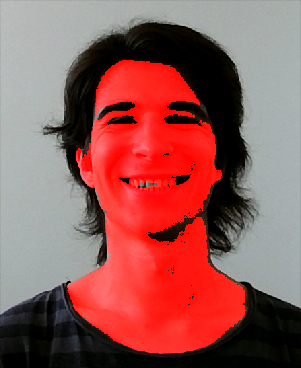
\includegraphics[scale=0.4]{skin_detection_heuristic}
            \label{fig:skin_detection_heuristic}
        \end{figure}
